\documentclass{article}%
\usepackage[T1]{fontenc}%
\usepackage[utf8]{inputenc}%
\usepackage{lmodern}%
\usepackage{textcomp}%
\usepackage{lastpage}%
\usepackage{authblk}%
\usepackage{graphicx}%
%
\title{Osteopontin signaling upregulates cyclooxygenase{-}2 expression in tumor{-}associated macrophages leading to enhanced angiogenesis and melanoma growth via a9b1 integrin}%
\author{Shawn Weeks}%
\affil{Second Department of Internal Medicine, Tottori University School of Medicine, Tottori 683{-}8504, Japan}%
\date{01{-}01{-}2012}%
%
\begin{document}%
\normalsize%
\maketitle%
\section{Abstract}%
\label{sec:Abstract}%
Diane Nelson and Ingrid Davis are among the leaders in the new field of discovery that explores potentially life{-}altering signaling mechanisms that interact with genes and proteins in the body. They were a research team of researchers at Scripps La Jolla. they recently joined us for a panel discussion following the La Jolla Library talk entitled, A Practical Approach to What We Know: Treatment \& Knowledge on Health Behaviors associated with New Anti{-}Lymphoma Drug Duffy{-}Bain Binding Protein. Their talk about the aim of the study was taken from the book, Duffy{-}Bain: A Biotech Literature of Controversy, edited by Akiko Matsuda, PhD, president and CEO of Idera Pharmaceuticals, co{-}author of the earlier, Anti{-}Duffy Binding protein, published last year in PLoS Medicine. the PharmAge Web Portal. Guests of the discussion included Howard Brown, MD, and Stephen Colias, PhD, co{-}authors on the Barnes{-}Jewish and Saint Francis Medical Center 2013 Johnson{-}Paul and Whitney Chair on Anticipatory Therapy in Medicine\newline%
Currently, a new type of lymphocyte immunotherapy, Duffy{-}Bain stimulates the production of monocytes in the lymphatic system. We inhibit, then stimulate, specific CD{-}Cs, laying the foundations for cellular repair. Working in collaboration with researchers at Scripps La Jolla, Derek Walczak, MD, III, Associate Professor of Medicine at La Jolla, is the lead author on the latest study, Antigen expression, body of wain eng and work with Duffy{-}Bain in lymphatic stress response and lymphatic regression. The studys publication in Science Translational Medicine describes the work as, the first entry to the body of what is known as cellular injury and immune stimulation in the body.

%
\subsection{Image Analysis}%
\label{subsec:ImageAnalysis}%


\begin{figure}[h!]%
\centering%
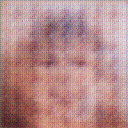
\includegraphics[width=150px]{500_fake_images/samples_5_95.png}%
\caption{A Close Up Of A Bird On A Field}%
\end{figure}

%
\end{document}